\def\layersep{3cm}
\def\outsep{0.7cm}
\def\dy{1.25}

\begin{tikzpicture}[draw=black!50, node distance=\layersep, font=\sffamily]
    \tikzstyle{node}=[circle,fill=black,minimum size=2pt,inner sep=0pt]
    \tikzstyle{block}=[draw=black,rectangle,fill=none,minimum size=1cm, inner sep=0pt]
    \tikzstyle{annot} = []

	\node[node] (xc) at (0, 0 cm) {};
    \node[block, text width = 2cm, align= center, right of=xc] (DSP) {$h[n], H(z)$};
	\coordinate[right of=DSP] (yc) {};
		
    \path[->, >=stealth, shorten >= 0pt] (xc) edge (DSP);
    \path[->, >=stealth, shorten >= 0pt] (DSP) edge (yc);
    
	\onslide<1-2|handout:1>{
		\node[block, draw=none, scale=0.5] (tx_signal1) at ($(xc.north) + (-1.5cm, 3cm)$) {\resizebox{12cm}{!}{\begin{tikzpicture}
\begin{axis}[
width=4.52in,
height=3.56in,
scale only axis,
separate axis lines,
every outer x axis line/.append style={white!15!black},
every x tick label/.append style={font=\color{white!15!black}},
xmin=0.00,
xmax=20.00,
ymin=-1.00,
ymax=1.00,
xlabel={},
ylabel={},
xmajorgrids,
ymajorgrids,
every outer y axis line/.append style={white!15!black},
every y tick label/.append style={font=\color{white!15!black}},
legend style={draw=white!15!black,fill=white,legend cell align=left}]
\definecolor{matlabColor1}{rgb}{0.000000,0.000000,1.000000}
\addplot [color=matlabColor1, only marks, line width=1.5pt, mark=*, mark size=2pt, forget plot]
table[row sep=crcr]{
	0 1 \\
	1 6.1232e-17 \\
	2 -1 \\
	3 -1.837e-16 \\
	4 1 \\
	5 3.0616e-16 \\
	6 -1 \\
	7 -4.2863e-16 \\
	8 1 \\
	9 5.5109e-16 \\
	10 -1 \\
	11 -2.4499e-15 \\
	12 1 \\
	13 -9.8034e-16 \\
	14 -1 \\
	15 -2.6948e-15 \\
	16 1 \\
	17 -7.3541e-16 \\
	18 -1 \\
	19 -2.9398e-15 \\
	20 1 \\
};

\end{axis}
\end{tikzpicture}}};
		\node[below = 0.5mm of xc] {$x[n] = \cos(\omega_0n)$};	
		\node[below = 0.5mm of yc] {$y[n] = x[n]\ast h[n]$};
	}
	\onslide<2|handout:1>{
		\node[block, draw=none, scale=0.5] (rx_signal1) at ($(yc.north) + (1.5cm, 3cm)$) {\resizebox{12cm}{!}{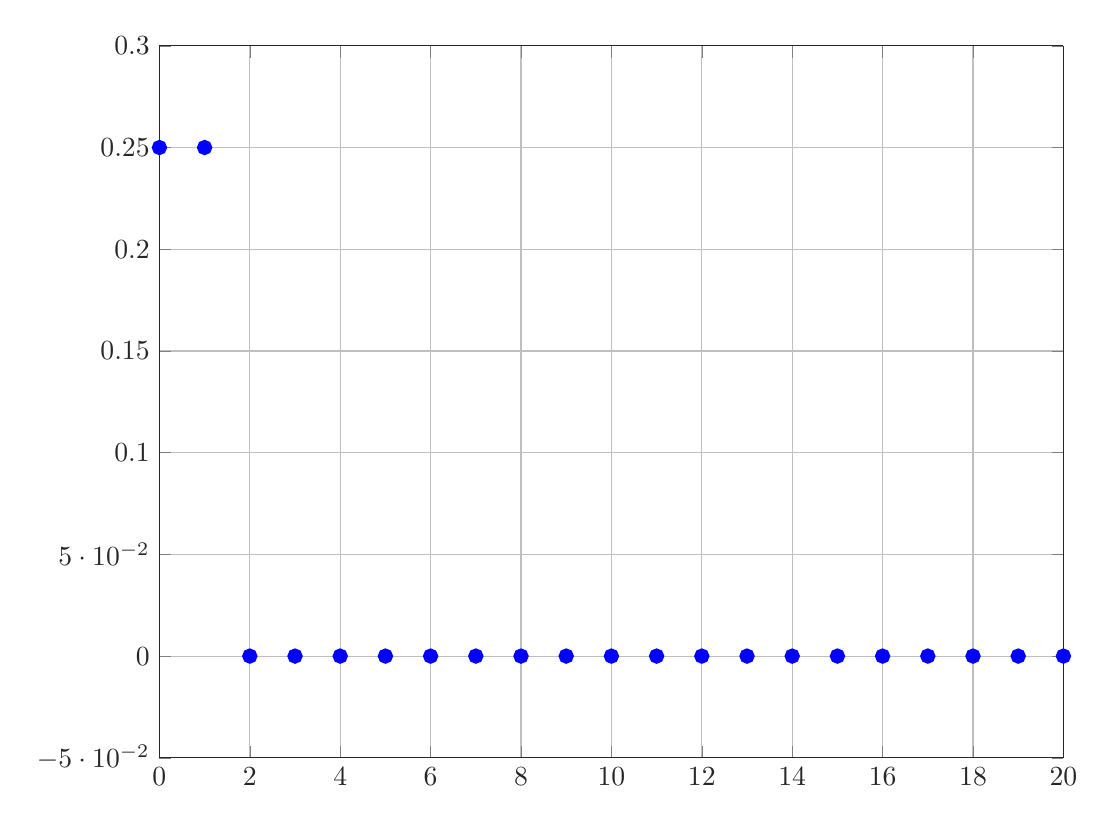
\begin{tikzpicture}
\begin{axis}[
width=4.52in,
height=3.56in,
scale only axis,
separate axis lines,
every outer x axis line/.append style={white!15!black},
every x tick label/.append style={font=\color{white!15!black}},
xmin=0.00,
xmax=20.00,
ymin=-0.05,
ymax=0.30,
xlabel={},
ylabel={},
xmajorgrids,
ymajorgrids,
every outer y axis line/.append style={white!15!black},
every y tick label/.append style={font=\color{white!15!black}},
legend style={draw=white!15!black,fill=white,legend cell align=left}]
\definecolor{matlabColor1}{rgb}{0.000000,0.000000,1.000000}
\addplot [color=matlabColor1, only marks, line width=1.5pt, mark=*, mark size=2pt, forget plot]
table[row sep=crcr]{
	0 0.25 \\
	1 0.25 \\
	2 0 \\
	3 -4.5924e-17 \\
	4 0 \\
	5 2.1029e-17 \\
	6 0 \\
	7 -5.1645e-17 \\
	8 0 \\
	9 2.675e-17 \\
	10 0 \\
	11 -5.0146e-16 \\
	12 -4.996e-16 \\
	13 -8.5571e-16 \\
	14 -8.6042e-16 \\
	15 -9.2351e-16 \\
	16 -8.8818e-16 \\
	17 -8.4999e-16 \\
	18 -8.6042e-16 \\
	19 -9.2923e-16 \\
	20 -8.8818e-16 \\
};

\end{axis}
\end{tikzpicture}}};
	}

	\onslide<3-4|handout:2>{
	\node[block, draw=none, scale=0.5] (tx_signal1) at ($(xc.north) + (-1.5cm, 3cm)$) {\resizebox{12cm}{!}{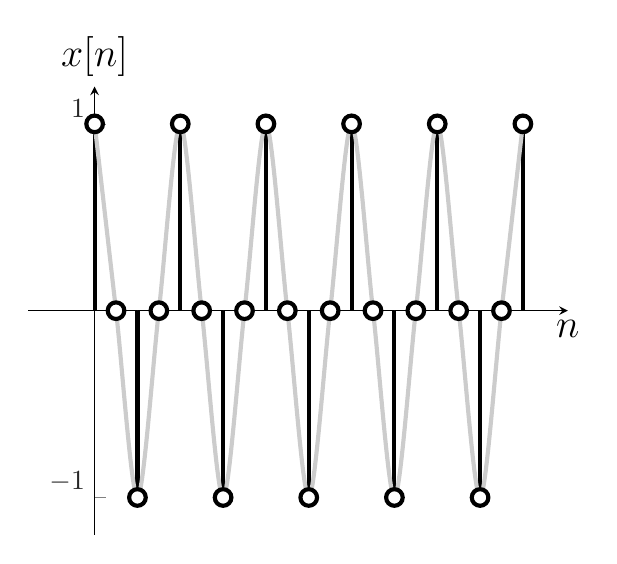
\begin{tikzpicture}
\begin{axis}[
axis lines*=middle,
enlargelimits = true,
ymin=-1,
ymax=1,
xmin=-1,
xmax=20,
axis line style={->,>=stealth},
xlabel={\Large $n$},
ylabel={\Large $x[n]$},
yticklabel style = {yshift=0.2cm},
xticklabel style = {yshift=-0.1cm},
every axis x label/.style={
	at={(ticklabel* cs:1)},
	anchor=north,
},
every axis y label/.style={
	at={(ticklabel* cs:1)},
	anchor=south,
},
ytick={-1, 1},
xtick=\empty,
every outer y axis line/.append style={white!15!black},
every y tick label/.append style={font=\color{white!15!black}},
legend style={draw=white!15!black,fill=white,legend cell align=left}]
\addplot [ycomb, mark=*, fill=white, mark options={scale=1.5, fill=white}, line width=1.5pt, forget plot]
table[row sep=crcr]{
	0 1 \\
	1 6.1232e-17 \\
	2 -1 \\
	3 -1.837e-16 \\
	4 1 \\
	5 3.0616e-16 \\
	6 -1 \\
	7 -4.2863e-16 \\
	8 1 \\
	9 5.5109e-16 \\
	10 -1 \\
	11 -2.4499e-15 \\
	12 1 \\
	13 -9.8034e-16 \\
	14 -1 \\
	15 -2.6948e-15 \\
	16 1 \\
	17 -7.3541e-16 \\
	18 -1 \\
	19 -2.9398e-15 \\
	20 1 \\
};

\addplot [smooth, black!20, line width=1.5pt, forget plot]
table[row sep=crcr]{
	0 1 \\
	1 6.1232e-17 \\
	2 -1 \\
	3 -1.837e-16 \\
	4 1 \\
	5 3.0616e-16 \\
	6 -1 \\
	7 -4.2863e-16 \\
	8 1 \\
	9 5.5109e-16 \\
	10 -1 \\
	11 -2.4499e-15 \\
	12 1 \\
	13 -9.8034e-16 \\
	14 -1 \\
	15 -2.6948e-15 \\
	16 1 \\
	17 -7.3541e-16 \\
	18 -1 \\
	19 -2.9398e-15 \\
	20 1 \\
};

\end{axis}
\end{tikzpicture}}};
	\node[below = 0.5mm of xc] {$x[n] = \cos(\omega_0n)$};	
	\node[below = 0.5mm of yc] {$y[n] = x[n]\ast h[n]$};
	}
	\onslide<4|handout:2>{
		\node[block, draw=none, scale=0.5] (rx_signal1) at ($(yc.north) + (1.5cm, 3cm)$) {\resizebox{12cm}{!}{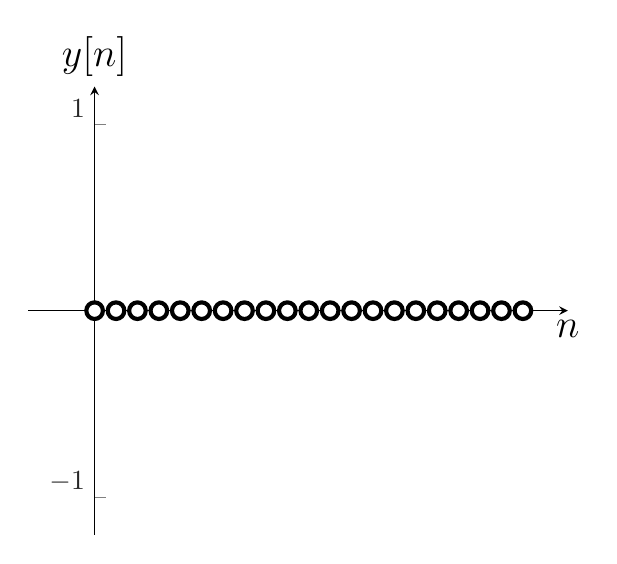
\begin{tikzpicture}
\begin{axis}[
axis lines*=middle,
enlargelimits = true,
ymin=-1,
ymax=1,
xmin=-1,
xmax=20,
axis line style={->,>=stealth},
xlabel={\Large $n$},
ylabel={\Large $y[n]$},
yticklabel style = {yshift=0.2cm},
xticklabel style = {yshift=-0.1cm},
every axis x label/.style={
	at={(ticklabel* cs:1)},
	anchor=north,
},
every axis y label/.style={
	at={(ticklabel* cs:1)},
	anchor=south,
},
ytick={-1, 1},
xtick=\empty,
every outer y axis line/.append style={white!15!black},
every y tick label/.append style={font=\color{white!15!black}},
legend style={draw=white!15!black,fill=white,legend cell align=left}]
\addplot [ycomb, mark=*, fill=white, mark options={scale=1.5, fill=white}, line width=1.5pt, forget plot, domain=0:20, samples=21] {0};

\end{axis}
\end{tikzpicture}}};
	}


\end{tikzpicture}